\documentclass[aps,pre,amsmath,amssymb,floatfix,onecolumn,notitlepage,10pt]{revtex4-1}
\usepackage{graphicx,isomath}
\usepackage[colorlinks=true,linkcolor=blue,citecolor=blue,urlcolor=blue,pdfborderstyle={/S/U/W 1}]{hyperref}

\begin{document}

\title{Continuation of oscillatory localized states: two case studies}
\author{Zachary G. Nicolaou}
\date{\today}

\maketitle
\tableofcontents

\section{Introduction}
Complex patterns of synchrony can emerge in networks of coupled oscillators.  Recently, for example, a myriad of localized traveling chimera states were reported to occur in the ring of Janus oscillators (a remarkably simple generalization of the Kuramoto model) \cite{2019_Nicolaou}. Localized oscillatory states have also been noted in heterogeneous arrays of parameterically-driven pendula \cite{2021_Nicolaou_1}, which have also been of interest because of their anharmonic responses in the study of classical time crystals \cite{2021_Nicolaou_2}.

In other contexts, localized steady-state solutions are known to occur through universal snaking bifurcations. The snaking bifurcations of steady-state solutions in the one-dimensional Swift-Hohenberg equation, for example, can be understood through the winding geometry of homoclinic and heteroclinic orbits \cite{2006_burke, 2009_beck}. In higher spatial dimensions, snaking bifurcations of steady-state solutions are known to exhibit  more complex features, such as multiple snaking branches and isolas \cite{2019_bramburger,2020_bramburger}.


The study of snaking bifurcations has previously focused on steady-state solutions to ordinary and partial differential equations, but patterns of synchrony typically exhibit nonstationary dynamics, which represents a different higher-dimensional problem.  There is a potential for the geometric interpretation of steady state snaking bifurcations to extend to snaking of limit cycle or chaotic attractors. However, to the best of the author's knowledge, no such connections have been made.  Furthermore, since limit cycles can exhibit both period doubling and torus bifurcations in additional to fold bifurcations, they have the potential to exhibit novel snaking phenomena not possible for steady state solutions, which only exhibit fold and Hopf bifurcaitons.

The purpose of these notes is to investigate whether the emergence of localized patterns of synchrony can be related to previous understanding of steady-state snaking bifurcations. We note how symmetry constrains the solutions and bifurcations in the parametrically-driven pendulum array and the ring of Janus oscillators, and we numerically continue the observed attractors through a complex series of bifurcations.

\section{Gap solitons in parametrically-driven pendula}
\subsection{Previous observations}
\begin{figure}[hbt]
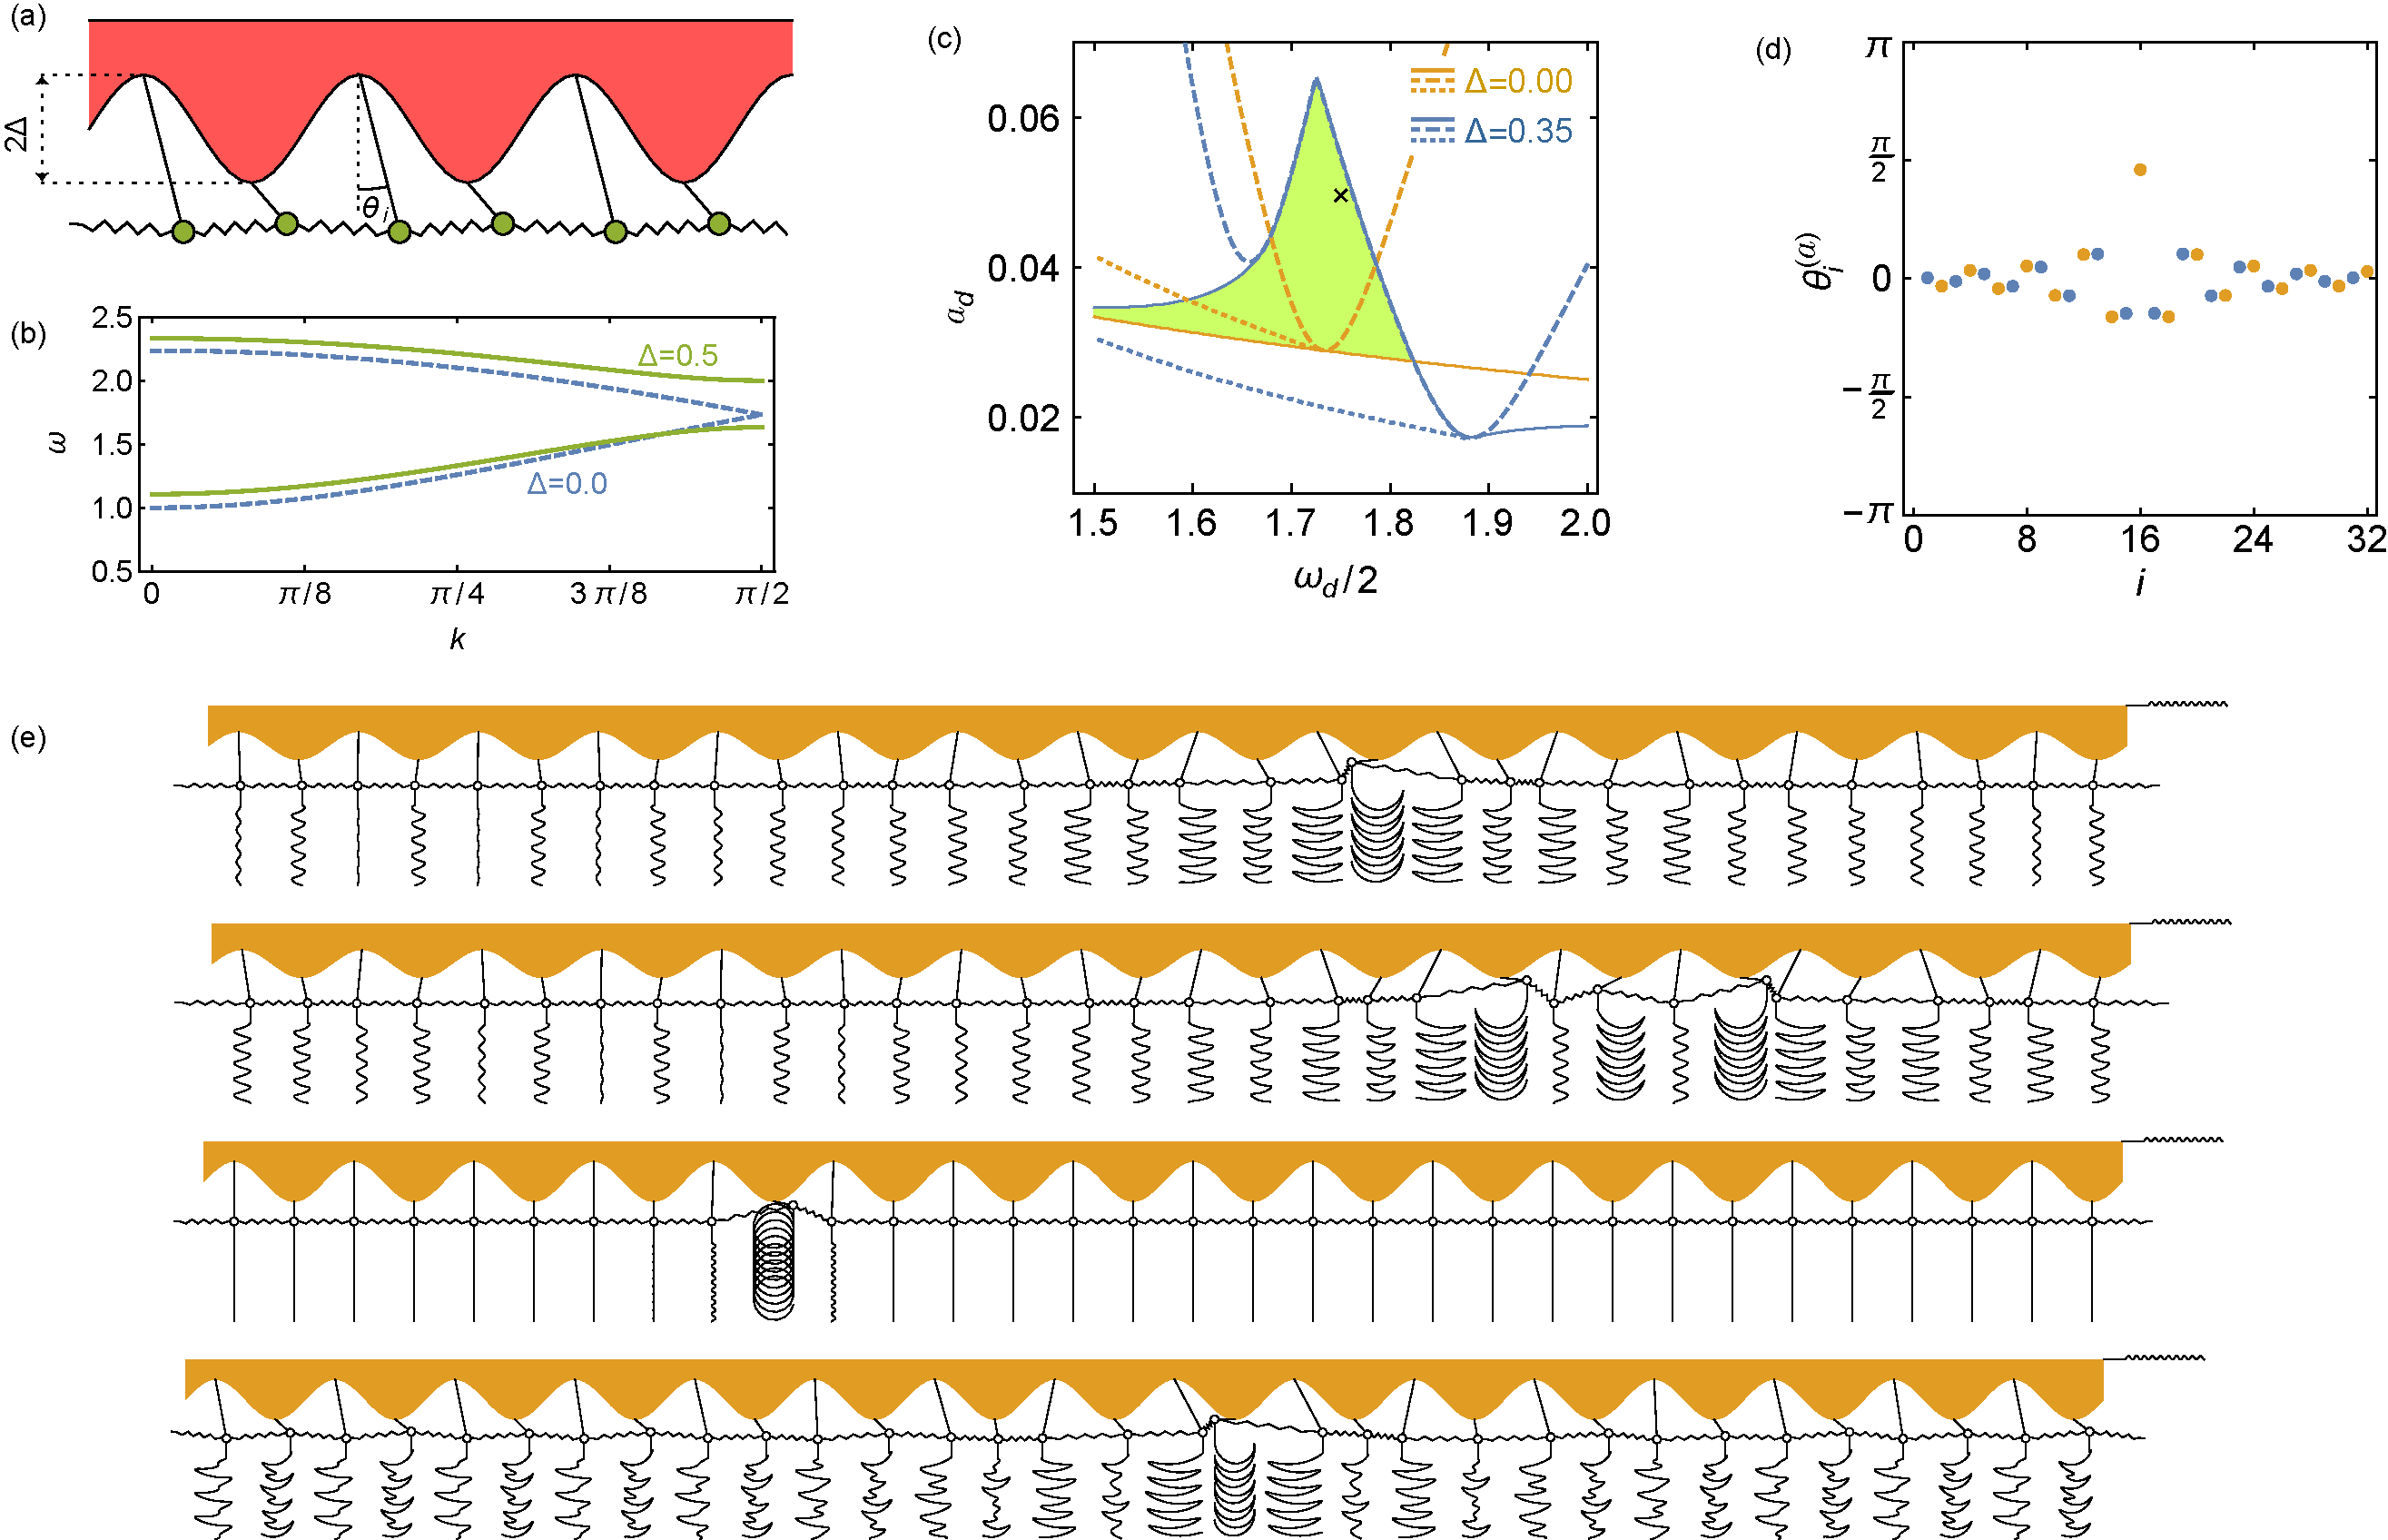
\includegraphics[width=\columnwidth]{pendula}
\caption{Gap solitons in parametrically-driven pendula. \label{fig1}}
\end{figure}
Recent studies on heterogeneity-homogenenized states \cite{2021_Nicolaou_1} and anharmonic classic time crystals \cite{2021_Nicolaou_2} employed a model describing a parametrically-driven array of pendula with alternating lengths [Fig.~\ref{fig1}(a)]. In this model, the angles $\theta_n$ and $\phi_n$ of the $n$th long and short pendulum evolves according to
\begin{align}
M \ddot{\theta}_n &= -\eta \dot{\theta}_n-M \frac{g - 4\Delta +  a_d \omega_d^2 \cos(\omega_d t)}{1+\Delta}\sin(\theta_n) +\kappa \frac{1-\Delta}{1+\Delta} \left[\sin(\phi_n-\theta_n) + \sin(\phi_{n-1}-\theta_n)\right],  \label{pendula1} \\
M \ddot{\phi}_n &= -\eta \dot{\phi}_n-M \frac{g + 4\Delta +  a_d \omega_d^2 \cos(\omega_d t)}{1-\Delta}\sin(\phi_n) +\kappa \frac{1+\Delta}{1-\Delta} \left[\sin(\theta_n-\phi_n) + \sin(\theta_{n+1}-\phi_n)\right], \label{pendula2}
\end{align}
where $\Delta$ is the alternating length scale, $a_d$ is the driving amplitude, and $\omega_d$ is the driving frequency, and we fix the damping to $\eta=0.1$, the gravitational acceleration to $g=1$, the mass to $M=1$, and the coupling spring constant to $\kappa=1$. For concreteness, we assume there are a finite number $N$ pairs of pendula, and we employ periodic boundary conditions with $n=N+m$ identified with $n=m$.

The behavior of the array dramatically differs for $\Delta=0$ and $\Delta>0$, since a band gap opens in the dispersion relation of the undriven array for $\Delta>0$ [Fig.~\ref{fig1}(b)]. In the limit of infinitely many pendula, the band-gap opening corresponds to a region of stability in the driven array for which heterogeneity stabilizes the homogeneous state consisting of stationary, vertically-hanging pendula [Fig.~\ref{fig1}(c)]. When the homogeneous state is perturbed by finite-amplitude disturbances in the stabilized region, it is possible to excite oscillatory states in which the swinging amplitude is localized [Fig.~\ref{fig1}(d)]. A plethora of such localized states coexist for sufficiently large $\Delta$, with varying configurations of localization centers [Fig.~\ref{fig1}(e)]. For yet larger $\Delta$, even more localized states emerge than previously identified [Fig.~\ref{fig1}(f)], including states with rotating pendula and non-periodic states related to co-resonance phenomena.

\subsection{Continuation equations}
In order to regularize the $2\pi$-discontinuity corresponding to rotations in the angular representation, we employ a complex representation $z_n=e^{i\theta_n}$ and $w_n=e^{i\phi_n}$ for numerical continuation. Since the model is second order in time, we also introduce the auxiliary momenta variables $p_n = (1+\Delta)\dot{\theta}_n$ and $q_n=(1-\Delta)\dot{\phi}_n$ to derive first-order equations.  Lastly, we introduce a auxiliary complex variable $Z$ evolving according to the Stuart-Landau equation, which will act as the periodic drive on the pendula. We then consider the complex equations of motion
\begin{align}
\dot{z}_n&=iz_np_n/(1+\Delta)+\gamma(1-|z_n|^2)z_n \label{cpendula1} \\
M\omega_d\dot{p}_n&=-\eta p_n - (Mg+a_d\omega_d^2\frac{Z+Z^*}{2}+4\kappa\Delta)\frac{z_n-z_n^*}{2i} +\kappa(1-\Delta)\frac{(w_n+w_{n+1})z_n^*-(w_n^*+w_{n+1})z_n}{2i} \label{cpendula2} \\
\dot{w}_n&=iw_nq_n/(1-\Delta)+\gamma(1-|w_n|^2)w_n \label{cpendula3} \\
M\omega_d\dot{q}_n&=-\eta q_n-(Mg+a_d\omega_d^2\frac{Z+Z^*}{2}-4\kappa\Delta)\frac{w_n-w_n^*}{2i} +\kappa(1+\Delta)\frac{(z_n+z_{n-1})w_n^*-(z_n^*+z_{n-1})w_n}{2i} \label{cpendula4}\\
\dot{Z}&=iZ+\gamma(1-|Z|^2)Z. \label{cpendula5}
\end{align}

The auxiliary variable $Z$ is decoupled from the other equations and quickly relaxes to the limit-cycle attractor $Z=e^{i\tau}$, where $\tau\equiv \omega_d t$ is the non-dimensional time. Thus, the terms $(Z+Z^*)/2$ in Eqs.~\eqref{cpendula2} and \eqref{cpendula4} reduce to $\cos (\omega_d t)$, which acts as the parametric driving term. Denoting the polar coordinates as $z_n = \rho_n{\mathrm e}^{i\theta_n}$ and $w_n = \eta_n{\mathrm e}^{i\phi_n}$, a straightforward change of variables leads to the polar equations of motion for the amplitudes $\dot \rho_n = \gamma \rho_n \left(1-\rho_n^2\right)$ and$\dot \eta_n =  \gamma \eta_n \left(1-\eta_n^2\right)$. Note that the amplitude dynamics decouples from the phases and are attracted to the fixed points $\rho_n=1$ and $\eta_n=1$.  Thus, we can initialize the equations with unit amplitudes, and the addition of the auxiliary dimensions in the complex representation is irrelevant.  The phase equations reduce to a non-dimensionalized version of the pendulum array Eqs.~\eqref{pendula1}-\eqref{pendula2}. The major advantages of the complex representation for numerical continuation is that, unlike the phases, these variables remain bounded in time even for rotating solutions, and the limit-cycle attractors are periodic in the complex variables. We express Eqs.~\eqref{cpendula1}-\eqref{cpendula5} in Cartesian coordinates to continue the resulting system of $6N+2$ real equations in AUTO.

\subsection{Discrete symmetries}
The pendulum array is invariant under the reflection $\pi$ given by $(\theta_n',\phi_n') = \pi(\theta_n,\phi_n) \equiv (\theta_{N-n},\phi_{N-n-1})$ and the rotation $R$ given by $(\theta_n',\phi_n')=R(\theta_n,\phi_n)\equiv(\theta_{n+1},\phi_{n+1})$. In studying the stability of the homogeneous state, the translational symmetry allows the Floquet multipliers to be parameterized by a spatial wavenumber $q$, and (co)resonance is only possible between degenerate wavemodes with the same wavenumber \cite{2021_Nicolaou_2}. Although they cannot mix and produce coresonance, the reflection symmetry guarantees that the Floquet modes corresponding to $q$ and $-q$ are degenerate. This poses a challenge to numerical continuation, since there are degenerate Floquet exponents which go unstable during bifurcations. Equivariant bifurcation theory accounts for such degenerate bifurcations in symmetric systems, and continuation methods for symmetric limit-cycle solutions have been proposed \cite{2006_Wulff}. Unfortunately, AUTO does not (yet) accommodate symmetry degeneracies for general systems, and some bifurcations can go undetected.  Fortunately, the $q=\pi$ and $q=0$ wavemodes do not have negative counterparts, since they lie at the center and the edges of the first Brillouin zone, so AUTO is able to continue the period-doubling $q=\pi$ bifurcation corresponding to the band-gap relatively well. When other, symmetric solution branches bifurcate with the solution, however, some bifurcations are not detected.

\subsection{Numerical continuation}
\begin{figure}[htb]
\includegraphics[width=0.75\columnwidth]{penduladiagram.pdf}
\caption{Bifurcation diagram for the parametrically-driven pendulum array with $\omega_d=3.5$ and $\Delta=0.35$, with thick lines showing stable limit cycles and thin lines showing unstable limit cycles. \label{fig2}}
\end{figure}
We have continued the homogeneous and gap-soliton solutions that appear from random initial conditions with $a_d=0.05$ and $\omega_d=3.5$ in an array of $2N=16$ pendula in AUTO using Eqs.~\eqref{cpendula1}-\eqref{cpendula5}. For the continuation, we fix the driving frequency of $\omega_d=3.5$ and alternating length scale $\Delta=0.35$, and continue with respect to the driving amplitude. To visualize the solution branches, we employ the norms $r_1^2=\int\sum_n\sin(\theta_n)^2+\sin(\phi_n)^2 {\mathrm d}t$ and $r_2^2=\int\sum_n\dot{\theta}_n^2+\dot{\phi}_n^2 {\mathrm d}t$ [Fig.~\ref{fig2}]. Stable (unstable) solutions are shown as thick (thin) lines. The homogeneous state corresponds to the green horizontal lines with $r_1=r_2=0$. This homogeneous state goes unstable in a period-doubling bifurcation PD1. All other limit cycle solutions in Fig.~\ref{fig2} have a period twice the driving period. The initial period doubling bifurcation is sub-critical and corresponds to a spatial wavenumber $q=\pi$, with an unstable swinging branch emerging for lower driving amplitudes [thin green line]. This branch exhibits a limit point LP1, but does not becomes stable when it turns around here. This is because an additional branching bifurcation SBP occurs on the solution branch prior to the limit point. This is a symmetric bifurcation point that is undetected by AUTO, with multiple real Floquet exponents simultaneously passing through zero. Consequently, two other unstable branches emerge from this symmetric bifurcation. One of the solution branches becomes stable [thick orange line] after turning around in a second limit point LP2. This solution branch corresponds to a localized gap-soliton centered around a single localized swinging pendulum. The gap solution undergoes various other branching and torus bifurcations, leading to a complicated tangle of solution branches, with stability occasionally re-emerging.

\section{Traveling chimeras in ring networks of Janus oscillators}
\subsection{Previous observations}
\begin{figure}[hbt]
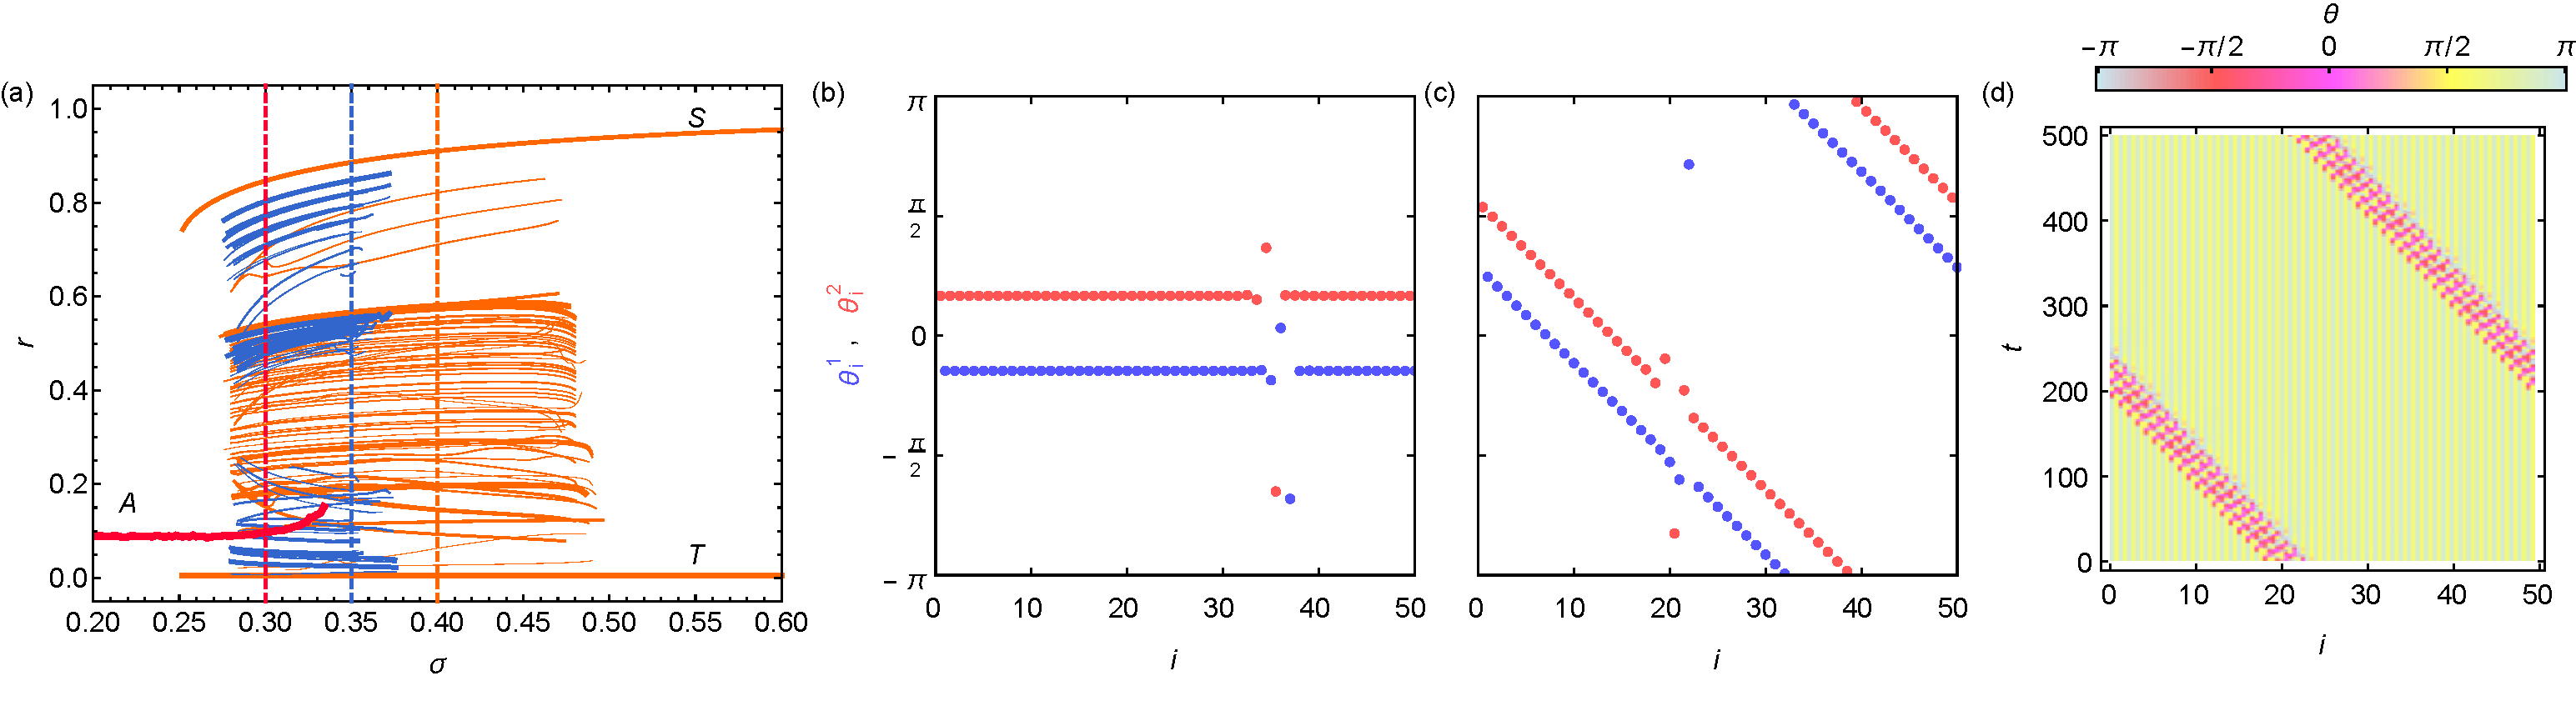
\includegraphics[width=\columnwidth]{janus}
\caption{Traveling chimeras in the ring of Janus oscillators. \label{fig3}}
\end{figure}
The introduction of antiferromagnetic order to the Kuramoto model results in a parsimonious model that exhibits a surprising variety of complex dynamics known as the ring of Janus oscillators \cite{2019_Nicolaou}.  Here, we aim to study the bifurcations in the ring of Janus oscillators, defined by the equations
\begin{align}
\dot{\theta}_n &= \omega/2 + \beta\sin(\phi_n - \theta_n) + \sigma \sin(\phi_{n+1}-\theta_n), \label{janus1}\\
\dot{\phi}_n &= -\omega/2 + \beta\sin(\theta_n - \phi_n) + \sigma \sin(\theta_{n-1}-\phi_n), \label{janus2}
\end{align}
with $n=N+m$ identified with $n=m$ for periodic boundary conditions. We fix the frequency gap to $\omega=1$ and the internal coupling strength to $\beta=0.25$. Previous studies have shown that random initial conditions relax to a plethora of attracting solutions for intemediate coupling strength $\sigma$. Quasistatically varying $\sigma$, these attracting solutions continue over a range of $\sigma$ [Fig.~\ref{fig3}(a)]. Investigating  a snapshot of the phases in these solutions [Fig.~\ref{fig3}(b)] reveals an orderly, synchronized portion of oscillators that coexist with a small number of asynchronous oscillators, with various amounts of phase twisting and configurations of synchronous/asynchronous groups.  These attractors break the symmetry in the network of identical, identically-coupled oscillators and are thus chimera states.   The asynchronous group of oscillators is not fixed, however, but travels at a constant speed around the ring [Fig.~\ref{fig3}(c)], so the attractors are traveling chimera states.

\subsection{Continuation equations}
For the sake of numerical continuation, we again consider complex equations
\begin{align}
\dot z_n &= z_n\left( i\omega/2 + \beta/2\left(w_nz_n^*-z_nw_n^*\right) + \sigma/2\left(w_{n+1}z_n^*-z_nw_{n+1}^*\right)\right) + \gamma\left(1-z_nz_n^*\right)z_n, \label{eom1} \\
\dot w_n &= w_n\left( -i\omega/2 + \beta/2\left(z_nw_n^*-w_nz_n^*\right) + \sigma/2\left(z_{n-1}w_n^*-w_nz_{n-1}^*\right)\right) + \gamma\left(1-w_nw_n^*\right)w_n. \label{eom2}
\end{align}
Again, the amplitude dynamics are decoupled from the phase dynamics and become irrelevant, while the phase dynamics reduce to Eqs.~\eqref{janus1}-\eqref{janus2}. In Cartesian coordaintes, Eqs.~\eqref{eom1}-\eqref{eom2} then result in $4N$ real equations whose solutions we will numerically continue.

\subsection{Discrete symmetries}
The ring of Janus oscillators is not reflection symmetric for $\sigma \neq \beta$, since the coupling between $\theta$ and $\phi$ variables has an inherent chirality. Instead, Eqs.~\eqref{janus1}-\eqref{janus2} posses at least two discrete parity-reversing symmetries. First, the ring is invariant under the time/parity reversal $\pi_1$ given by $(\theta_n',\phi_n',t') = \pi_1(\theta_n,\phi_n,t) \equiv (\pi+\phi_{N-n},\theta_{N-n},-t)$. Since this map reverses the direction of time, stable solutions are mapped to unstable solutions under $\pi_1$.  Second, the ring is invariant under the parity/sign reversal $(\theta_n',\phi_n',t') = \pi_2(\theta_n,\phi_n,t) \equiv (-\phi_{N-n},-\theta_{N-n},t)$. Since the direction of time is preseved by this map, the map $\pi_2$ takes stable solutions to other stable solutions.  Note that the parity/sign reversal symmetry leaves the Kuramoto order parameter $r\equiv \left\lvert \sum_n e^{i\theta_n}+e^{i\phi_n}\right \rvert$ invariant as well (so there are two branches of solutions corresponding to each line in the bifurcation diagrams below). Composition of the two parity symmetries gives a time/sign reversal symmetry $\pi_3$ defined by $(\theta_n',\phi_n',t')=\pi_3(\theta_n,\phi_n,t)\equiv(\pi-\theta_n,-\phi_n,-t)$. Lastly, the ring is invariant under discrete rotations defined by $(\theta_n',\phi_n',t')=R(\theta_n,\phi_n,t)\equiv(\theta_{n+1},\phi_{n+1},t)$, taking the periodic boundary conditions into account.

\subsection{An additional continuous symmetry}
Since the phase equations depend only on phase differences, the equations are invariant under global phase rotations $\theta_i\to\theta_i+\psi$ and $\phi_i\to \phi_i+\psi$.  This means that limit cycle attractors and fixed point attractors will have a neutrally stable perturbation direction corresponding to phase rotations. For limit cycle attractors, with the additional neutral perturbation corresponding to time shifts $\theta_i\to\theta_i+\epsilon\dot{\theta_i}$ and $\phi_i\to\phi_i+\epsilon\dot{\phi_i}$, there will be two unit Floquet multipliers for all parameter values, rendering all points singular in the pseudo-arclength continuation method employed by AUTO. To fix this problem, we could change variables to include the conserved quantity $\Theta = \sum_n \left(\theta_n + \phi_n\right)$ in the Janus ring. In such coordinates, the conserved quantities will decouple from a reduced system, and we can study stability in the reduced system instead.  A slightly simpler reduction in the ring of Janus oscillators can be made by moving into a reference frame that rotates at the speed of, say, oscillator $z_0$. Define quantities $\tilde{z}_n = z_n/z_0$ and $\tilde{w}_n = w_n/z_0$ (whose phases are, respectively, $\theta_n-\theta_0$ and $\phi_n-\theta_0$).  Then $\dot {\tilde z}_n = \dot z_n / z_0 - \left(z_n/z_0\right)\left( \dot z_0/z_0\right)$ and $\dot {\tilde w}_n = \dot w_n / z_0 - \left(w_n/z_0\right) \left(\dot z_0/z_0\right)$. Assuming (wlog) that $z_0$ is initialized with $z_0=1$, we then have upon substituting into Eqs.~\ref{eom1}-\ref{eom2}
\begin{align}
\dot {\tilde z}_n &= i{\tilde z}_n\left(  \beta/2\left({\tilde w}_n{\tilde z}_n^*-{\tilde z}_n{\tilde w}_n^* - {\tilde w}_0+{\tilde w}_0^*\right) + \sigma/2\left({\tilde w}_{n+1}{\tilde z}_n^*-{\tilde z}_n{\tilde w}_{n+1}^* - {\tilde w}_1+{\tilde w}_1^*\right)\right) + \gamma\left(1-{\tilde z}_n{\tilde z}_n^*\right){\tilde z}_n, \label{janus_rot1}\\
\dot {\tilde w}_n &= i{\tilde w}_n\left( -\omega + \beta/2\left({\tilde z}_n{\tilde w}_n^*-{\tilde w}_n{\tilde z}_n^* -{\tilde w}_0^*+{\tilde w}_0 \right) + \sigma/2\left({\tilde z}_{n-1}{\tilde w}_n^*-{\tilde w}_n{\tilde z}_{n-1}^* - {\tilde w}_1+{\tilde w}_1^*\right)\right) + \gamma\left(1-{\tilde w}_n{\tilde w}_n^*\right){\tilde w}_n. \label{janus_rot2}
\end{align}
It is straightforward to continue of the $4N-2$ real equations in the Cartesian forms of Eqs.~\eqref{janus_rot1}-\eqref{janus_rot2} using AUTO.

\subsection{Time-shift reductions for chimera states}
The chimera state solutions in the ring of Janus oscillators are traveling waves. We cannot change to moving spatial coordinates since the lattice is discrete, but we can instead consider the time-delayed coordinate $\tau_n = t - \nu n$ for oscillator $n$, where $1/\nu$ is the velocity. We can enact a reduction if we assume that the oscillator dynamics are identical in their respective time-delayed coordinates (i.e., the variables depend on time only through the invariant coordinate $\tau_n$). Additionally, the space translational invariance and the invariance under global phase rotations enables a reduction, which we call the cluster-twisted traveling wave ansatz: $z_n(t) = e^{i\eta n}\left(X_{n\,\text{mod}\,q}(t-\nu n)+iY_{n\,\text{mod}\,q}(t-\nu n)\right)$ and $w_n(t) = e^{i\eta n}\left(U_{n\,\text{mod}\,q}(t-\nu n)+iV_{n\,\text{mod}\,q}(t-\nu n)\right)$, where $q$ denotes the number of clusters and $\eta$ is twist parameter, and $\nu$ is, again, the velocity.  Inserting this ansatz into Eqs.~\eqref{eom1}-\eqref{eom2}, taking $X_m + iY_m = e^{i\Theta_m}$, $U_m+iV_m=e^{i\Phi_m}$, and ignoring the (transient) amplitude dynamics, we find a set of $2q$ time-shift equations
\begin{align}
\dot{\Theta}_m(\tau) &= \omega/2 + \beta\sin(\Phi_m(\tau)-\Theta_m(\tau)) + \sigma\sin(\Phi_{m+1\, \text{mod}\, q}(\tau-\nu) -\Theta_m(\tau)-\eta), \label{timeshift1} \\
\dot{\Phi}_m(\tau) &= -\omega/2 + \beta\sin(\Theta_m(\tau)-\Phi_m(\tau)) + \sigma\sin(\Theta_{m-1\, \text{mod}\, q}(\tau+\nu) -\Phi_m(\tau)+\eta). \label{timeshift2}
\end{align}
Given a chimera state from numerical simulations, we can attempt to fit $\eta$, $\nu$, and $q$ in order to reduce the solution to a limit-cycle solution of Eqs.~\eqref{timeshift1}-\eqref{timeshift2} with period $T$. On a ring of $N$ Janus oscillators, periodicity in space implies that $N\nu = p T$ for some integer $p$, so that $\nu = pT/N$. In the limit of large $N$, the chimera solutions correspond to a localized disturbance in $\Theta_m(\tau)$ and $\Phi_m(\tau)$, with asymptotic $\tau \to \pm \infty$ behavior corresponding to a steady state of $q$-clustered synchrony with twisting rate determined by $\eta$. In principle, these localized solutions may undergo snaking bifurcations, leading to chimera states with groups of co-traveling asynchronous regions. The time delay here complicates this analysis somewhat both theoretically and numerically, however.

\subsection{Numerical continuation}
\begin{figure}[htb]
\includegraphics[width=0.9\columnwidth]{janusdiagram.pdf}
\caption{Bifurcation diagrams for traveling chimera states in the ring of Janus oscillators. \label{fig4}}
\end{figure}
We have continued chimera branches in a ring of $N=8$ Janus oscillators in AUTO. Figure \ref{fig4} shows the results of this continuation.  We find that the attracting chimera state solutions all undergo bifurcations for both increasing and decreasing $\sigma$, but they do not connect with each other in our continuation. The numerics are limited because the period of the limit cycles [Fig.~\ref{fig4}(a)] typically becomes very large as the continuation continues in both directions. Because AUTO uses a fixed number of collocation points, the increasing period implies that the dynamics are eventually poorly resolved by the numerics. By examining the  Kuramoto order parameter [Fig.~\ref{fig4}(b)], we can also see that most of the limit-cycle chimeras turn around at limit points for $\sigma>0.25$, such as the point labeled SLP. Inspection of the Floquet exponents reveals that all the Floquet exponents become neutral simultanously at SLP. Furthermore, the parity-time reversal symmetry $\pi_1$ maps the stable green solution to the unstable green solutions. Thus, the solution becomes $\pi_1$-invariant at the limit point, and these points are actually symmetric branching points which are not appropriately detected by AUTO. Other solutions may emerge from such points as well.

In addition to the limit-cycle solutions, Eqs.~\eqref{janus1}-\eqref{janus2} possess various cluster-twisted steady-state solutions, which can be found which can also be numerically continued. We continued a few of these solutions for $q=1$ and $q=2$ clusters with a twisting parameter of $\eta=0$ [Fig.~\ref{fig4}(c)].  Most of the steady-state solutions are unstable, except for one with $q=1$ clusters corresponding to a synchronized state [thick blue line in Fig.~\ref{fig4}(c)]. Stable twisted synchronized states also exist with $\eta \neq 0$. The stable synchronized states also undergo symmetric limit point bifurcations, which go undetected in AUTO. These correspond to saddle-node on the invariant curve bifurcations (SNIC), in which a heteroclinic orbit between a saddle and a node coincides with a limit cycle at the bifurcation, and continues in the opposite direction of the fold [not shown]. This limit cycle corresponds to a remotely synchronized state in the ring of Janus oscillators which is neutrally stable and not attractive \cite{2019_Nicolaou}. The period of this neutrally stable limit cycle approaches infinity at the SNIC point. We see that in addition to the limit cycle, the saddle, and the node, several other unstable equilibria emanate from the SNIC point. For non-zero twisting number $\eta$, there are many more unsteady equilbria that emanate from twisted SNIC bifurcations as well, leading to an unwieldy number of unstable equilibria in the model.

\section{Discussion}
Our numerical investigations so far have been specific. For the array of parametrically-driven pendula, we should consider continuations with respect to the other problem parameters. A preliminary two-parameter continuation of $\omega_d$ and $a_d$ for the period-doubling bifurcations of the homogeneous state does coincide with the instability boundary determined by a problem-specific Floquet theory \cite{2021_Nicolaou_1,2021_Nicolaou_2}. We would also like to consider the bifurcations for differing $\Delta$. Can we observe a more orderly snaking bifurcation for smaller $\Delta$ where the gap solitons first emerge? And can we continue or understand the localized state connected with the anharmonic response that emerge for larger $\Delta$, which may be either quasiperiodic or chaotic? For the ring of Janus oscillators, it seems likely that the traveling chimera limit cycles may undergo saddle-node bifurcations on the invariant curves of some of these steady cluster-twisted solutions, since the period of the chimera solutions appear to become infinite in Fig.~\ref{fig4}(a).  Can we make a quantitative numerical correlations of these bifurcations, despite the unwieldy number of steady cluster-twisted solutions?  For both systems, does increasing system size result in an increasing ladder of snaking bifurcations? How can we more systematically deal with the symmetric bifurcations leading to the localized states? Most importantly, do these examples represent a universal class of localized oscillatory phenomena?

\begin{thebibliography}{99}
\bibitem{2019_Nicolaou} Z. G. Nicolaou, D. Eroglu, and A. E. Motter. Multifaceted dynamics of Janus oscillator networks. \textit{Phys. Rev. X} \textbf{9}, 011017 (2019).
\bibitem{2021_Nicolaou_1} Z. G. Nicolaou, D. J. Case, E. B. Van der Wee, M. M. Driscoll, and A. E. Motter. Heterogeneity-stabilized homogeneous states in driven media. \textit{Nature communications} \textbf{12}, 4486 (2021).
\bibitem{2021_Nicolaou_2} Z. G. Nicolaou and A. E. Motter. Anharmonic classical time crystals: A coresonance pattern formation mechanism. \textit{Physical Review Research} \textbf{3}, 023106 (2021).
\bibitem{2006_burke} J. Burke and E. Knobloch. Localized states in the generalized Swift-Hohenberg equation. \textit{Phys. Rev. E} \textbf{73}, 056211 (2006).
\bibitem{2009_beck} M. Beck, J. Knobloch, D. J. B Lloyd, B. Sandstede, and T. Wagenknecht. Snakes, ladders, and isolas of localized patterns. \textit{SIAM Journal on Mathematical Analysis} \textbf{41}, 936-972 (2009).
\bibitem{2019_bramburger}J. J. Bramburger, D. Altschuler, C. I. Avery, T. Sangsawang, M. Beck, P. Carter, and B. Sandstede. Localized radial roll patterns in higher space dimensions. \textit{SIAM Journal on Applied Dynamical Systems} \textbf{18}, 1420-1453 (2019).
\bibitem{2020_bramburger}J. J. Bramburger, and B. Sandstede. Spatially localized structures in lattice dynamical systems. \textit{Journal of Nonlinear Science} \textbf{30}, 603-644 (2020).
\bibitem{2006_Wulff} Wulff, Claudia, and Andreas Schebesch. "Numerical continuation of symmetric periodic orbits." SIAM Journal on Applied Dynamical Systems 5, no. 3 (2006): 435-475.
\end{thebibliography}
\end{document}
